\documentclass[xcolor=dvipsnames, 14pt]{beamer} 
\usecolortheme[named=Brown]{structure} 
% \useoutertheme{umbcfootline}
\usetheme[height=10mm]{Rochester} 
% \usetheme{Rochester} 

\setbeamertemplate{items}[default] 
\setbeamertemplate{itemize subitem}[circle] % if you wnat a circle

\usepackage[spanish]{babel}
\usepackage[utf8]{inputenc}

\usepackage{graphicx}

\usepackage{color}
\usepackage{listings}
\lstset{ %
language=Prolog,            % choose the language of the code
breaklines=true,            % sets automatic line breaking
frame=single,               % Add a frame to listings.
basicstyle=\footnotesize,   % Font size.
}

\usepackage[absolute,overlay]{textpos}
\newenvironment{reference}[2]{%
  \begin{textblock*}{\textwidth}(#1,#2)
      \footnotesize\it\bgroup\color{gray!50!black}}{\egroup\end{textblock*}}
% 128mm×96mm

% items enclosed in square brackets are optional; explanation below
\title{Invisble.js}
\subtitle{Trabajo profesional de Ingeniería en Informática}
\author{
Martín Paulucci \\
Facundo Olano
}
\institute[UMBC]{
  Facultad de Ingeniería\\
  Universidad de Buenos Aires \\
}
\date{20 de Diciembre, 2013}

\newtheorem{codigo}{Código}

\begin{document}

%--- the titlepage frame -------------------------%
\begin{frame}[plain]
  \titlepage
\end{frame}

\begin{frame}{Arquitectura Web}
    \begin{center}
        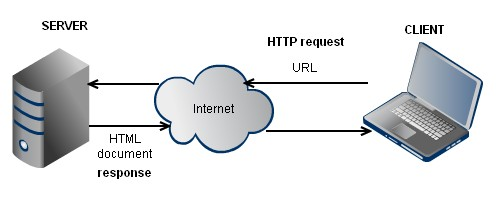
\includegraphics[width=\textwidth]{img/http.png}
    \end{center}
\end{frame}

\begin{frame}{Programación Web: Prehistoria}
    \begin{center}
        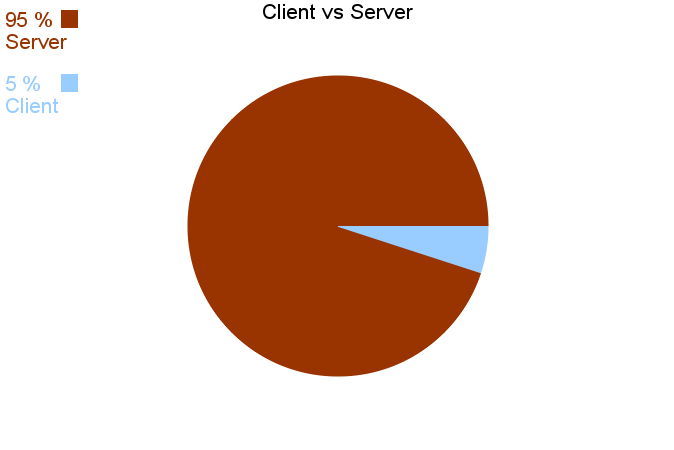
\includegraphics[width=\textwidth]{img/prehistoria.png}
    \end{center}
\end{frame}

\begin{frame}{Programación Web: Historia}
    \begin{center}
        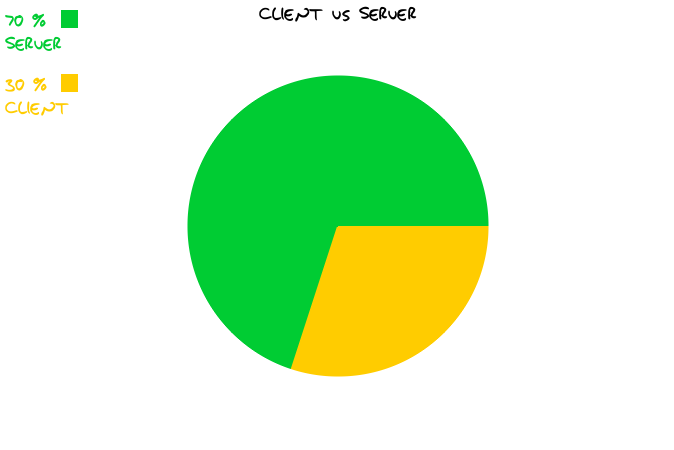
\includegraphics[width=\textwidth]{img/historia.png}
    \end{center}
\end{frame}

\begin{frame}{Programación Web: Actualidad}
    \begin{center}
        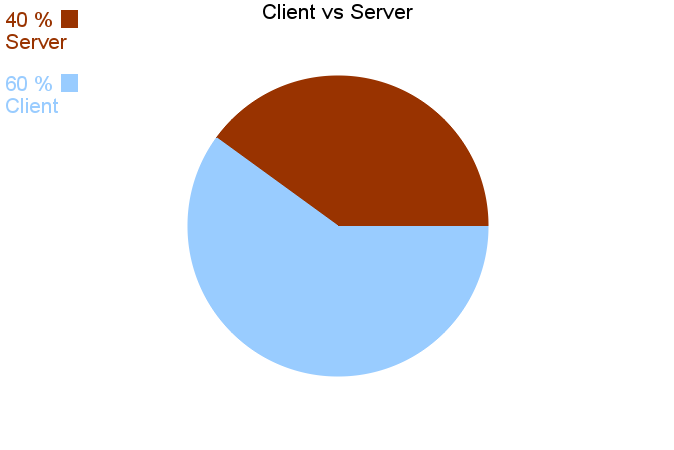
\includegraphics[width=\textwidth]{img/actualidad.png}
    \end{center}
\end{frame}

\begin{frame}{Problemas Actuales}
\end{frame}

\begin{frame}{Programación Web: Futuro}
\begin{reference}{4mm}{13mm}
``The best way to predict the future is to invent it.'' Alan Kay
\end{reference}

\begin{columns}
    \begin{column}{0.3\textwidth}
        \begin{itemize}
            \item Meteor
            \item Derby
            \item Invisible?
        \end{itemize}
    \end{column}
    \begin{column}{0.7\textwidth}
        \begin{center}
            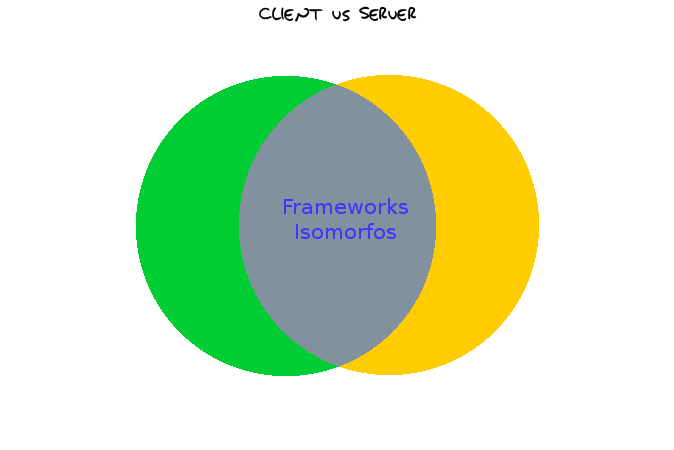
\includegraphics[width=\textwidth]{img/futuro.png}
        \end{center}
    \end{column}
\end{columns}

\end{frame}

\begin{frame}{Nuestro objetivo}
\begin{reference}{4mm}{13mm}
``Al buscar lo imposible el hombre siempre ha realizado y reconocido lo posible.'' Mijaíl Bakunin
\end{reference}

\end{frame}

\begin{frame}{Investigación}
\begin{reference}{4mm}{85mm}
``If you think it's simple, then you have misunderstood the problem.'' Bjarne Stroustrup
\end{reference}

\begin{columns}

\begin{column}{0.5\textwidth}
    \begin{itemize}
    \item CoffeeScript
    \item Server Push
        \begin{itemize}
        \item Log Polling
        \item SSE
        \item WebSockets
        \item socket.io
        \end{itemize}
    \item REST
    \item Templates
    \end{itemize}
\end{column}

\begin{column}{0.5\textwidth}
    \begin{itemize}
    \item node.js
        \begin{itemize}
        \item Express
        \item Derby
        \item Meteor
        \item Flatiron
        \end{itemize}
    \item Client MV*
        \begin{itemize}
        \item Backbone
        \item Angular
        \item Knockout
        \end{itemize}
    \end{itemize}
\end{column}

\end{columns}

\end{frame}

\begin{frame}{Prototipos Realizados}
\begin{reference}{4mm}{85mm}
``Hay que unir lo teórico a lo Real, lo ideal a lo Empírico.'' Juan Perón
\end{reference}

\begin{itemize}
    \item \emph Fodder : REST + SSE + Handlebars
    \item \emph drymodels : Node.js + Express + Backbone
    \item \emph Acekia : Node.js + Angular + CoffeeScript
\end{itemize}
\end{frame}

\begin{frame}{Arquitectura en Invisible.js}
\begin{reference}{4mm}{85mm}
``There's only one trick in software, and that is using a piece of software that's already been written.'' Bill Gates
\end{reference}

\end{frame}

\begin{frame}{Modelos en Invisible.js}

\end{frame}

\begin{frame}{Modelos en Invisible.js (2)}

\end{frame}

\begin{frame}{Invisible.js en acción}

\end{frame}

\begin{frame}{Invisible.js en acción (2)}

\end{frame}

\begin{frame}{Demo}
    \begin{center}
        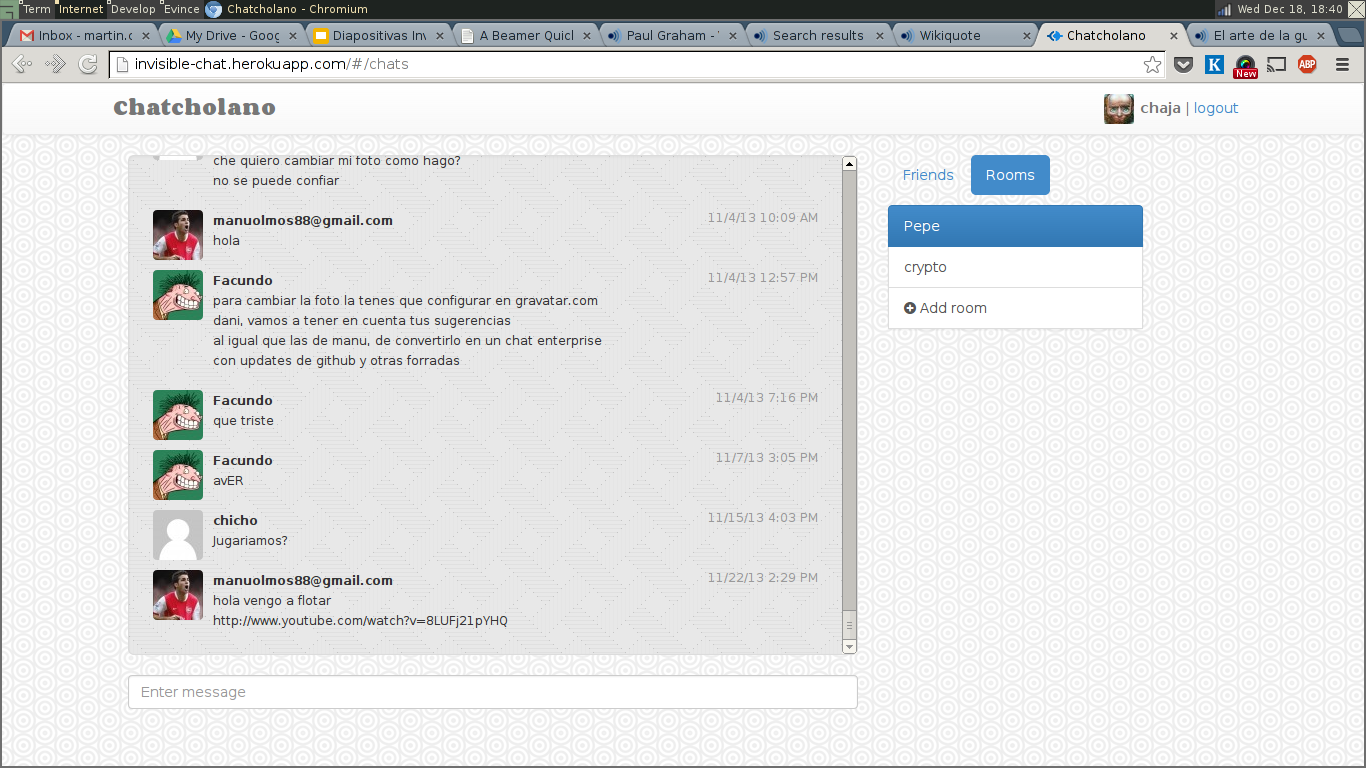
\includegraphics[width=\textwidth]{img/demo.png}
    \end{center}
\end{frame}

\begin{frame}{Conclusiones}
\begin{itemize}
    \item Desarrollo integral de un producto
    \item Objetivos cumplidos
    \item Sencillez y velocidad de trabajo
\end{itemize}
\pause

Trabajo futuro:
\begin{itemize}
    \item Seguridad
    \item Escalabilidad
    \item Desarrollo comunitario
\end{itemize}


\end{frame}

\end{document}
